\chapter{The Project: Notebooks from Trashed Papers}

%****************************************
% TODO proje ismi çok iyi değil onu bir adam etmek gerekli. 
% Notebook Project; from trash
% Notebooks from Trashed Papers
% Notebooks from trash
% Notebook Project: from trash to treasure
% Notebook Project: from trash
%........................................





% FROM Wild Art. quote taken from the television series `American Masters', Season 5, Episode 8, John Cage: I have nothing to say and I am saying it (aired on 17 September 1990).
\epigraph{The first question I ask myself when something doesn't seem to be beautiful is why do I think it's not beautiful? And very shortly you discover that there is no reason. If we can conquer that dislike, or begin to like what we did dislike, then the world is more open. That path ---of increasing one's enjoyment of life--- is the path, I think, we all best take: to use art not as self-expression, but as self-alteration; to become more open.}{\hfill---John Cage, \textit{Wild Art}, 2013}





In this chapter thesis project with the development progress of it will be explained in detail in the light of what has been discussed in previous chapters.

% Proje nedir, kısaca bahsetmek lazım. Projenin bileşenleri daha sonra detaylı bir şekilde anlatılacaktır. Ama önce nasıl geliştiğine bakalım.

% What I have write is here to cover the project can not be sufficient. Because it is not possible to say everything about this project. I wish that this work would allow different interpretation and readings. 

\comment{Research and the found samples of works helped a lot to shape my work. They provide me deeper understanding of the subject and what I am doing and they lead me during the development of the work.}





\section{Artist Statement}
(Collect, Save, Transform, Spread.)(Rescue, Revive.)

[Transform] With the help of art (and artistic practices) discarded things can find a place in the society. (By the help of artistic approach things can be gain new values and meaning even if they are discarded and excluded from daily life (or society).) With the help of art discarded things ---in the scope of thesis particularly paper trash--- can be transformed beyond the other industrial (or technological) methods. 

[Work] Converting disposal things to multiple usage (or anything that is durable as noted in the rubbish theory). Realizing the alternative lifes of trash beyond their defined one shot life. Giving attention to the things. \comment{Inquerying concepts and perceptions that are not cared.} The work aims to liberate the imagination and change the way people see the trash.

[LIFE PRACTICE, CHANGES ON PEOPLE] Actually (It is questioned that) the effects of working with trash to the life practice. Working with trash is a convergence of behavioral patterns (attitudes toward to trash) and art making. The process effects one's life and lifestyle. (But what type of interaction between life and art making process?) (This claim is the main driving force of my artwork which is part of a thesis.) Looking for things and meanings in the normal course of life.

[DISTANCE] The purpose is not to build a thing that is produced from discarded material to watch it from a distance. The important thing is to interact with it. Because it is already discarded (disgusting, abject, unattractive etc.) and general behavior avoid from it. This work must change it. It must call the viewer to interact with it. Trash must be accepted.

% Ersan hoca uzak seyretmek yerine etkileşime geçilmesini auranın kırılması olarak bakıyor. Performatif olması veya bir act olması zaten bunu kıran bir şey olabilir. Sanatsal eylem, performans kavramlarını araştırmak gerekli. Uzaktan seyredip hayranlık duymak yerine ilişkiye geçilen bir hale getirmek çöpü. Amaç bu aslında. Çöpü tekrar tanımak, onunla barışmak, onunla yaşamak. İşte bu yüzden bir eylem olabilir. Ya da yaşam pratiği. 

% Olay sadece böyle çöpten bir şeyler yapıp insanların seyretmesi değil, mühim olan onunla iletişime, ilişkeye geçmek. Yani zaten uzak durulan bir şey, onlardan bir şey üretildiğinde izleyici gene uzağında duruyorsa ne anlamı kaldı ki? İnsanlar bu işin aşamalarının bir parçası olmalılar.

[ACT, COMMUNICATION, COLLABORATION] In this work it is claimed that the process of transformation of trash can be treated as artistic act. In the production of notebooks people collected papers from different places and location. During the collection phase, they have also collected them from other people. Communication and collaboration played significant role in the progress. (With this communication and collaboration the approach to the trash is explored in different cases.)

[NEW RESOURCE] Junk(or trash) can be seen as a new resource that is fertile to new meanings, creations and aesthetics. Ignored and discarded nature of garbage, when rethought, becomes a fertile resource. Trash as a resource (as an artistic material). (City as a resource. Seeing the discarded items as a resource. Many artist approach to trash as resource. Some of them collect city discard, some of them tea cups, tea bags, discarded papers.)

% TODO new comer. [POTENTIAL, new resource]
% FROM Book: Recycled, Re-Seen: Folk Art from the Global Scrap Heap
[building new things from ruin] \comment{small amount of it} while most waste ends up in these unsanitary and unsightly landfills, some small percentage is reincorparated --- or recycled --- back into the economic and cultural system of the local population. Indeed, this is the power of rubbish as a category of possessable objects: it has within itself the potential of being discovered, retrieved, and transformed back into an object of greater or lesser durability. 

% Belki Chapter 3'e taşınabilir.
% [Resource, Potentials] I resurrect things that have been killed off... My work is all about the potential of materials — even when it looks like they've lost all possibilities. (Cornelia Parker) https://en.wikipedia.org/wiki/Cornelia_Parker

% TODO new comer. Statement or approach.
\comment{TRASH AND OTHER DISCARDED NOTIONS} From my point of view and approach in this thesis, trash is only one of the thing that is being discarded by humans and communities. There are lots of things that are being excluded such as homosexuals, trans, disabled peoples etc. Even if they are excluded, there is also life for them. 




% Not all waste is dirty, it not always dangerous, contagious or abject. \ldots waste might be quite useful in making time and in keeping time.


% Çöpe nasıl yaklaşak gerekli? Bu tezde sorulan sorulardan birisi bu.



%
%
\section{Development Progress of Work}
How does it start? How does it evolve in time? Important points that shaped the work\ldots This progress also reveals the how this work can be positioned among the other works. Choices, interpretations, approaches... Encountered problems. Experiments with the material.
% \comment{Tarihsel bir süreç mi yoksa bu işi bir araya getiren şeylerin nasıl bir araya geldikleri mi?}

It is not a fixed(static) project. It is evolved in time and affected from other artists' work, and gain meaning from research.

Before explaning the details of the work, it would be better how it was started, what is my approach to the trash and so on?





%
%
\textbf{How is it started?} As far as I know I collect things it is hard to say collecting started after an exact event or time but there are several memories that I remember. One of these (First of them) is from my primary school teacher. When I was third class my teacher give us a homework to bring colorful paper to make something(whatever it is I don't remember). The day after we bring some colorful paper but she did not. Instead of this she bring paper cut out from packages that are colorful, shinny and qualify. And I remember clearly that she suggest that same for us. Do not throw out packages, look for the useful parts and keep them to use later. \comment{Actually people collect things. There is nothing strange here. They collect what their needs. or they will need in the future. It is more different than just need. It is also self exploration. Feeling uncomfortable to buy simple things. I can make some of them. Looking for alternative, different feeling and texture.} 

\comment{I have remembered that we are covering our notebooks at school. Sometimes we also cover the books.}

\comment{Being under pressure of spirit of our age. Looking for the everytime most efficient way and best performance. Everything can be purchaseble... ready, easy to use, easy to throw away. no intimate relationships with items objects. By trasnforming the disposable items I establish a different connection between them. They are replaceable with the other one (Especially it can be seen in the works of TeaBagWork and PaperCoffeeCupWork).}





%
%
\textbf{What do I think about trash?} I need to clarify my approach to the trash, wasting and discarding. First point is that I am very uncomfortable to the action of discarding thing. I always think that by discarding this think I am missing something rather than getting rid of something. Sometimes because of the significant amount of residue from consumption from daily activities I became overwhelmed and to move on I need to leave behind them and move on. However almost it is never ending loop. (I believe that sometimes we need to break the loops to realize different meanings. To think outside the box, we need to behave outside of common habits. As I mentioned the discarding things are some of the loops that we are rare to behave like other way.) \textbf{What am I discarding?} To get rid of my load and move on. But for what? and also ought to be like that? (throw away them to same bin. (Some of people do not care too much bin and throw them whenever it is possible.)) Even if I discard some stuff I think that I am ignoring its potential and losing it. At that times I become very sad and feel very comfortable. I must have find to another place for it more suitable than a waste bin. At least I can give them someone else who can use it for own purposes. Do I really luxury of discard?

Significance of thinking outside of the box (about trash) is actually breaking the loops. You have to look at differently from your common perception. \textbf{Break the rules, break the loops} to realize the alternative. \comment{Even if the market gives many alternatives of commodities, why do people still seek the alternative? Is not is enough? What type of gap that industrial products can not fill the gaps. Neden tüm insanlara hitap etmiyor?}

[Making exploration.] One of the encouraging factor is to work on trash is to find (or explore) something different from someone else's discard. Because it is ignored by discarding and therefore undiscovered. Wait us to be discovered. and possiblely (as picasso mentioned) discovered again and again. \comment{Different people from different culture bring new interperation, but it is exist all of things.}

[Motivation.] I can not throw them away. When I throw them I became sad for them. I have to find something useful for it. (Failure of imagination, failure of making meaning) Even if I can not find it, I can pass it to another person who can make use of it for own purposes. We are humans that can able to make meanings, produce something, transform items. One of most developed species in the earth that produce and use tools. There is a lot of effort to produce objects and it seems that all this efforts are wasted. What I mention is not related about ultimate productivity. It is more close to being thoughtful, and taking responsibility of tools, items and objects that we are using. Rather than throwing out, creating a way that all are have chance to live together is much more close to my perception.

Beyond everything I make notebook for myself. I am showing(proving) that I can still make things. not everything is stolen from me. It does not steal anywhere.





%
%
\textbf{Paper}\todo{Konuyu biraz daha özetle.} [History] \todo{history of trash} The word paper comes from papyrus, the plant that was first used for making a medium for writing in ancient Egypt.

[Wide range of use] \paraphrase{Paper is an indispensable product throughout the world. Its primary use is as a medium for writing, essential for bureaucracy, education, communications, information storage, and in the spread of information. In addition, it is used for the packaging for transport and convenience of a wide range of items from food to industrial equipment. Paper also has specific technological uses, such as for filters and in art, home furnishings, and architecture, and it has a range of uses for hygiene purposes. Paper in several forms is consumed on a daily basis by each person in the Western world \cite{trafford2012paper}.} Having wide range of usage offers great diversity in order to make compositions. As they bring their old identity. 

[Uses of Paper] Paper has become the most ubiquitous product in the age of information. Such products often complete their journey from shop floor to garbage in a single day; for example, newspapers, print paper, packaging, lavatory paper, tea bags, transport tickets, price tags, shopping bags, flyers, leaflets, wrapping paper, napkins, and tissues. \comment{Traditionally, newspapers and magazines have been reused as paper for packing; covering different surfaces, such as  windows and furniture; and even as toilet paper.}

[Production, Recycling] \paraphrase{All types and qualities of paper share the same basic method of manufacture, including newspaper paper, print paper, and carton used for boxes. Paper made exclusively from wood is called virgin paper, while paper produced out of used paper that is re-pulped is called recycled paper. Recycling paper can greatly diminish demand for virgin fiber from wood. However, there will always be a demand for virgin paper because, although paper is thought of as a renewable resource, it cannot be recycled indefinitely. It can only be recycled four to six times, as the fibers get shorter and weaker each time. In addition, some virgin pulp must be introduced into the process each time to maintain the strength and quality of the fiber, so no matter how much is recycled, paper will always need some virgin fiber.}

\paraphrase{Post-consumer paper waste has to be manually sorted  into  different  types,  such  as  paperboard, office  paper,  and  newsprint.  Staples  are  removed with  a  magnet.  The  paper  is  chopped  into  small pieces  and  added  to  water  and  chemicals.  Denser objects that are not paper sink. Any inked or colored  papers  must  be  deinked  with  sodium  silicate or  sodium  hydroxide.  Some  paper  pulp  is  also bleached. The effluent of the pulping process, called “sludge,”  includes  chemicals,  inks,  clay  (from glossy paper), plastics, and short paper fibers. This sludge can be toxic and is landfilled or incinerated. When paper is recycled, the fibers break down and become shorter, requiring the input of virgin material. If virgin pulp is not added, the pulp can be used in lower-quality paper products, such as cardboard or newsprint.}

[Recycling, effects to the nature] \paraphrase{Paper is both biodegradable and a renewable resource, which means in consumption and waste terms, its environmental impact is relatively small compared to the many more-toxic and bulky waste products that are found in everyday garbage. However, the chemicals, water, and electricity used in its manufacture are considerable---and these are nonrenewable resources---and certain types of chemicals used in paper production are toxic. In addition, if waste paper is sent to a landfill, it releases carbon dioxide emissions. Further, forest resources are not always as renewable as one may like to think. These environmental impacts can be greatly reduced by recycling (paper being one of the most easily and cheaply recyclable products in everyday use) and by conscientious consumption practices.}

One of the key elements of the project is paper. Notebooks are made from trashed papers. Eve if they are discaeded they are still functional. There is a increasing intereset on papers because of  biodegrable nature of it(compared to plastic and nylon materials) [it is one of the reasons, not only.]. Therefore they are becoming more common. Mostly they are used as a package to keep safe and isolated commodities. Most of them  contain brand's logo and carry the identity of company. 

Papers that are mostly blank are used inside of the notebooks for writing. Others that have colorful logo and images on them are used as a cover for notebooks. \comment{I have also other type of packs such as Starbucks coffee packets.}

All packs are cleaned up. Because it is important that it needs to be safe to use. With mix of water and little bleach they are swabbed. 

[Why (package) paper?] Easy to collect. Easy to find. Thrown out even if it is good quality. Packaging materials are very widespread. Appropriate for painting and writing. Has a very short life time. Disposable, there are a lot of package outside. No need to carry it. Every place gives you package paper. 





%
%
\textbf{Collecting.} \comment{When I collect the papers under the dishes or food packages, people often think that it is disgusting and called them as dirty. However, it is very strange that the fat on the paper was previously what they are eating.}

One of the most found trash in my habitat is paper. I work at METU Technopolis, live at 100. yil which is the nearest settlement to METU and study at Bilkent. People live there commonly use paper and needs paper. Paper is nearly everywhere. Reusing the paper is not limited with recycling of it. There is a another ways of it. When we recycle them actually we again send away them and use it as we all know. (industrial papers and notebooks.) There is no richness here. Same type of paper. Produced after a industrial process. I collected them from my friends (people that have communicate often). Sometimes I collect them from trash bins and roads.

I have stored papers in my rooms. \todo{an image of storage of papers.}

% Why do I collect trash? Why paper? Who wants to keep trash? Who wants to re-see(re-visit) trash again? To use it again. 

% [Why do I collect trash?] Herkes neye ihtiyacı var ise onu toplar. Ben neden niçin topluyorum? Toplama sebepleri? Dönüştürme sebepleri. Neden sadece toplamakla yetinmiyorum. yani toplamak ile ayrıldığı noktalar nelerdir. Ben bir mana mı arıyorum? Yoksa kaybetmekten mi korkuyorum? Yeni kompozisyonlar oluşturmak istiyorum. Farklı karşımlar elde etmek istiyorum. Bir tür şaşırtmak durumu... Beklenmeyeni yapmak... En olmadık malzeme çöple çalışmak bu yüzden önemli benim için. 

% Bilinçsiz bir şekilde mi topluyorum yoksa, bilinçli bir şekilde.

[Organizing People] Well I actually follow very simple methods. I just talk them all. I explain what I did, ask for their help. Everyone actually approached positively and somehow they contributed the project. \todo{How does it differ from asking for their help? What type of meaning I add here?}

% [İnsanları işe dahil etmekle ilgili.] Bu işin olması için ben insanlardan bir şeyler yapmalarını istiyorum. Yani aslında kendimde yapabilirim ama neden insanları da dahil ediyorum? Buradaki en önemli amaç değiştirmek dönüştürmek, sadece çöpü dönüştürmek yetmez, insanların fikirlerini de deönüştürmek gerekmek. ve bu bir süreç işi (şart mı tek bir yöntem bu mu?) İnsanlar nasıl değişir diye sormak gerekir o zaman. İnsanların değiştiğini dönüştüğünü gerçekten nasıl ölçeceğim ki? 





% CROWDSOURSING, CITIZEN SCIENCE
% In view of the diversity of online crowdsourced art projects, as illustrated by the examples cited so far, it is useful to map out this artistic trend by developing a comprehensive and multidimensional typology of online crowdsourced art. Table 1 organizes this classification according to a set of multiple criteria. (But this one can be used at introduction, but it is too long to fit on introduction. Maybe select works by giving prominence to some of the features. So the approach to the trash is going to be introduced and also it is reveals the what i am doing in this context.) (A Typology of Online Crowdsourced Art. Diye bir örnek var aslında benzer bir şekilde bu trash içinde yapılabilir.) 

% In the words of Jeff Howe (2006b), the Wired columnist who coined this term in June 2006, \quotes{crowdsourcing represents the act of a company or institution taking a function once performed by employees and outsourcing it to an undefined (and generally large) network of people in the form of an open call}. The vital elements that qualify an outreach strategy as crowdsourcing are, according to Howe, the use of the open call format and the reliance on a large network of potential workers. Although in some cases there is a material reward for the best contributions, the existence of financial incentives is not a required feature in crowdsourcing. Because of the diversity of its applications, crowdsourcing continues to be a disputed term in both the scholarly literature and the popular press; Howe’s original definition is, in this sense, a helpful delineation of its practical sphere.

% The value of crowdsourcing lies in the collective intelligence of the contributors. Pierre Levy (1997) describes this concept as “a form of universally distributed intelligence, constantly enhanced, coordinated in real time, and resulting in the effective mobilization of skills” (p. 13). The question of collective intelligence—and its potential efficiency in various practical settings—has received much attention in both academia and journalism. Researchers studying team performance generally agree that, under the right circumstances and with appropriate motivation, large groups of people can work together and harness their collective intelligence to achieve efficient results (Benkler, 2006; Rheingold, 2002; Surowiecki, 2004). Nevertheless, artistic creativity is different from innovation and intelligence, and it requires a unique set of skills and sensibilities as well as a particular type of cultural capital; if we admit that crowds can have collective intelligence, do they also have collective creativity in an artistic sense?

% All these pages are rescued and with their [hi]story they are separated from unused new produced blank sheets and notebooks. They are not bought, not gift. They are found. They are accepted. One of the most creative medium is paper and pencil. Chance given to the people through this work.

% However, in view of its reliance on the artistic contribution of a large pool of usually anonymous participants, this type of art raises important questions about notions of collective creativity, authorship, collaboration, and the shifting structure of artistic production in the new digital environment. It is well studied area. Pick a method here. Transforming trash with collaboration.

% As curator Andrea Grover notes, “having the audience become co-creators is not a new impulse”; the Internet simply offered a new platform to accomplish this goal (Strickland, 2011, para. 5).

% Here this question can be raised about why this type collaboration. Another option can be working together with people on a table. Creating things at that time and transforming the objects here. Possibly the connection to the people will more realistic and intense. However same things can be succeed on the internet at some level. 

% While crowdsourced art challenges the traditional role of the artist, it simultaneously redefines the conventional function of the public, turning them from passive receivers into engaged producers. (This totally a new area to discuss, I'm going to summarize and introduce concepts and debates. How are they support my work and how they are give way to me?)

% This article therefore aims to fill these critical gaps by analyzing the practice of online crowdsourced art within a framework of collective creativity and participation theories. Principally, my interest is in answering two key questions. What is crowdsourced art and how can it be classified? And how does the structure of the artwork determine the degree or significance of participation?

% TODO: Umberto Eco's Open Work






[Criters, rules] There are some rules defines the frame of collecting act. Paper must be trash or going to be trashed. 

\textbf{Collected Materials.} There are different papers and packages are used to produce notebooks. 

\todo{Tüm buradaki resimleri appendixe eklemek gerekli, hatta bunlar sitede de olacaklar.}

\begin{description}
  \item[Burger King packages] are collected from the office where I work. At launch time, some of the colleagues order the meal from Burger King. The package of the meal is collected and used as a cover of notebooks.
  \item[Starbucks packages] are colled from my supervisor, office and my friend. Especially my supervisor and friend saved and collected them from their friends. They are used as a cover of notebooks.
  \item[Modshifters papers] that are covered on table and at the end of the day they are cut out and throw away. I go this place many times and every time questioned what they are doing to the papers. One of my visit we stay there at a late time and catch the garson collecting the old papers and prepearing tables to the next customer or day. I ask him to give me and he kindly accepted. From this paper I covered [x] notebooks. All of them contains track of people who sit down there. I do not know them and I am not sure that the paper that they are sit down turned to such a thing. 
  \item[Varuna Gezgin]
  \item[Graduation banner]
  \item[Tea bags]
  \item[Banka sıra fişleri]
  \item[Elginden gelen kağıtlar]
  \item[Bilkent kağıtları]
\end{description}

%  \begin{figure}[ht]
%      \centering
%      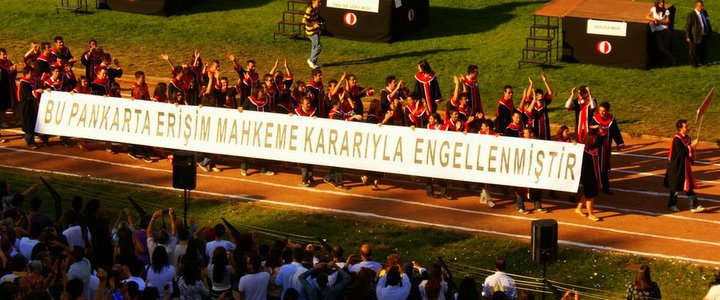
\includegraphics[height=6cm]{project_graphics/banner1.jpg}
%      \caption{Banner}
%      \label{fig:Banner_1}
%  \end{figure}

\begin{figure}[h!]
  \centering
  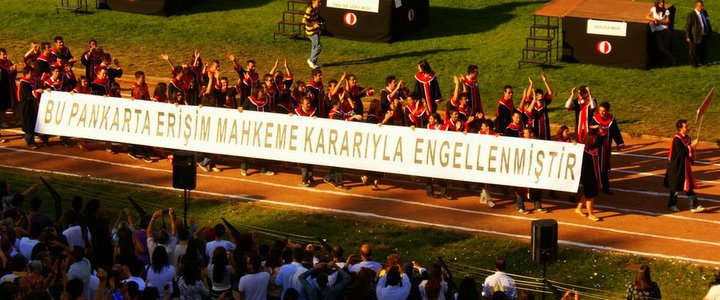
\includegraphics[width=1\textwidth]{project_graphics/banner1.jpg}
  \caption{Banner}
  \label{fig:Banner_1}
\end{figure}

% Collecting
% [Everywhere, everytime, Life practice.] En başta bahsettiğim everywhere, everytime aslında collecting ile çok yakından ilgili. Bu toplama işlemi normal hayatın içine sızıyor(infiltrate the life). 

% There is also strong relationship with the collecting discarded stuff and archeologies of waste. 

% TODO new comer
% WHO OWNS TRASH? kısmı benim işimde sorgulanabilir, ya da ünlülerin trashlerini inceleyen adam kısmında ele alınabilir. Orada aslında başkalarının trashlerinin insanlar hakkında neler anlattığını çok güzel anlıyoruz.
\comment{ANALOGY Between landfill and graveyards. WHOSE TRASH?} \quotes{There’s a relationship between graveyards and landfills, one that makes us uncomfortable, Zubiaurre explained. \quotes{What is happening to trash is what is going to happen to us. We’re all going to end up in a dump, and we’re going to decompose. That’s the ultimate destiny of humankind, and we don’t want to face that.} Trash is also regarded differently, depending on where you live. Last year, an undergrad in Zubiaurre’s honors collegium seminar went to a poor neighborhood and scavenged through people’s trash; no one cared, Zubiaurre said. But when the same student went to Beverly Hills to go through trash, the police were nearly called. \quotes{Who decides what is public and what is private? How come trash becomes highly private in a rich neighborhood, but truly disposable in a poor neighborhood?} Zubiaurre said.} \cite{zubiaurre2015trash}


%
%
\textbf{Transforming.} I turned them to notebooks. Actually I use them for my self. While I was using of them, I am very proud. I am studying nearly more than twenty years and I have always need for notebooks and use them. It is some sort of passion for me notebooks. Because I always admire notebook beautifully design or uniquely designed. I collect them whenever I find and most of the time I only save them for later use. 

% What I tried during this progress: Wrap out the trees, because I think that most of the materials that I collected are package papers. Well I somehow package the trees again. not to carry them but to raise awareness. Yani benim amacımı en iyi anlatacak olan şey nedir? Aslında ben burada defterden gidip bunu anlamlandırmaya çalıştım. Dolayısıyla deneyerek deftere nasıl ulaştım da ziyade defterden başlayıp nasıl tekrar defterde karar kıldığımı anlatan bir hikaye olabilir? Yani bu çok da şart olmayabilir bir diğer yandan da? Developlement of work? Nasıldı nereye geldi? How my project evolved? And this also explains how it is relates with the research. Because the reasearch is shaped the project also. Which part of the project shaped by the project? Not thinking in the ecological perspective. Raised questions also mature the project? For example zizek suggest that to find spirutuality and aesthetics to the trash, and for me? 

Actually I have been collecting same materials that are used in my project before the thesis work. In my mind there is always a belief\todo{objective olmalı...} that I can I find something useful for them. (In that time my main evaluation was to create useful object for my need.) Later it turned to an artwork. Before the thesis I also produce the notebooks for myself. However what is changed in thesis. First my approach to the trash is a little bit deeper. What is added to the notebooks. I started to use also used papers. for the cover of the notebook, I use more different materials. more close to collage. production method changed. and I started to collect different things, from different places. My realization increased. I organized my close friends and others to collect or save their trash for me. I discovered some points. their differences. 

Because I already do it. So What I didn't change it. It is the best one or no to change it. I love idea of carrying notebook with near of you. I have also save my notebooks. I don't throw away them. A notebook is actually is a work of you. It carries your signature. It is one of best gift to give someone. Because it is a combination of your work and the other peoples works. It is co-authored work. Actually there is also a part of people who throw away this peace. Actually the best part of it the transformation is not finishes after my creation of notebook. It continues with the usage of it. How it turned to is not actually uncertain. Therefore it is very appropriate of my idea that transforming trash is increases the diversity.

[What is different from industrial notebooks?] Handmade, from trash. an alternative to other versions. every one have different stories, they are different in visuals (but the others are also different.) What makes them different is not clear actually. Does it have to be different? Yes. The production method is different. You pay no money. There is different with gift notebooks from companies. This notebooks call to you change the destiny of trash together. 

[Why covering notebooks?] They are all package paper, already used as carry things and this work it has used again for the same purpose (but in different connection, this time trash is bound to the notebook). Trash is used to cover the papers. Cover is the most visible part of the notebook and book. Therefore trash becomes most visible part of the produced item. What is the function of cover? It gives ideas about what is inside, distinguishes from other things, protect it.

[Artistic tactics] Here I followed some tactics to accomplish my purposes. Easy to carry while traveling. Small notebooks. Placing them to their routes. 

% Notebooklar insanın yanında kolayca taşınabildiği için aslında bir yandan fikri yaymak için idea. Zaten showing off'un ne kadar önemli olduğu rubbish theoryde söylenmişti.

% [Standartlar, Dönüştürme seviyesi] endüstriyel standartlar, kaplar ve kağıtlar hep bir şekilde bir birleriyle boyut olarak uyuşuyorlar. İlk başlarda kesip biçmeye daha çok ihitiyaç duyarken zamanla basit katlamalar işimi görmeye başladı. Ne kadar az müdahele bulunursam aslında o kadar çok geldiği yerin özelliklerini o kadar çok temsil ediyordu. Bu da benim hoşuma gidiyordu. Kolaj mantığı işte abi. Ne kadar çok değiştirmek dönüştürmek istiyorsun. Burda şöyle bir durum var. çöpleri hiç tanınmayacak bir hale de getirebilirsin. Bu şekilde kimse onların farkına bile varmaz. Ya da neredeyse olduğu gibi kullanırsın. Yani uygulanan dönüştürmenin derecesi çok önemli burada.

% TODO new comer
the question of who owns these discards is not trivial. \cite{zimring2012encyclopedia}





%
%
\textbf{Exhibiting.} Starting point is to stack the notebooks onto the each other, and there are some ideas like putting them inside a waste bin to re-do the action of throwing away. Again the purpose is to find a way that to shock people, surprise them. After ward somehow they should understand that these notebooks can be taken. \comment{I set up makets and try some installations of it. Take photo it. listed them here.}

\todo{images are here.}

I imagine a exhibition environment and place notebooks at that place. Different placement are tried. All of them are look like sculptural. I have insert no special meaning as sculpture to this object an I also I am afraid that people does not close them to the notebooks and look them away. which I do not want. 

Aim is to spread the idea by making something useful from trash. Increase diversity, activate (or encourage) people to embrace the trash.

[Why in the public space?] To reach more audience. Actually the audience is out of the art galleries. They are walking in the streets. Putting them to next to people is much more effective. It is not visible and nearly it is hided from society. It is dirty. Removed from the society. There is a effort to hide them away. However in this project it is again showed to the society. Because it is revisited and reclaimed. 

% TODO
% [Why giving away?] Felix Gonzales Torres, Unlimited Editions.
% TODO insanlar bu defterleri alsınlar.




%
%
\section{Parts of project (or final work)}
The project introduced in this thesis have different parts. Each of them are connected to have relation with and support the other. Different parts also enable us that different level of integration to the project. 





%
%
\subsection{Notebooks}
Mixing(juxtaposing) materials is main method in the production process. I combine different papers and packages. I try to generate every possible combination. For some of them I establish the connection but for the others the connection is not obvious but it is not obligatory. Because trash is state where you can find meaning through the trash or material later. 

Every notebook has numbers and with this numbers it can be tracked down when it was produced and which materials are used production of it.

There are notebook series that have a name. Here are the name of notebooks and their story:

\begin{description}
\item[Puzzle.] Because it is cut out from very big and long banner (which is carried at graduation ceremony at METU, 2011). Every piece was a part of bigger banner. At that time there are serious debates about freedom on the internet. Most of the website are banned from the decision to the courts and they were not accessible. (Access to this banner is blocked by a court decision.) In Middle East Technical University there is a tradition that in graduation ceremony people walk through in the stadium and greet to the tribunes. With this event they carry some banners to express their feelings and criticize some realities in the country. This one of them. It is carried by students (new grads of Computer Engineering) The slogan decided by among the students and before the ceremony I printed out the slogan to carried out as many people as it can and easy to readable from the people who seat at the tribunes. After the ceremony I could not throw away this banner. I do not know what to do it, it is very big actually to store but I could not. I think that I will figure out later. Maybe I can use it as a draft paper. But is it worth to cut out this all long banner etc. Also to strengthen the banner and to prevent to tear while carried by the many people we are tape it from its boundaries. In other words some of the areas can not appropriate for writing. When I decided to this topic I remembered to this banner. It is stands in a corner in a dusty way. Now it is time use it. It waited very log time and it is time to revive again. Currently In turkey the problem of banning web-sites continues. Event it can said that people do not surprises when a website is blocked by the courts. It can be turn be a paper that people can freely express their ideas and feeling onto the it. Cut out them to the smaller pieces and make them as notebooks. They are part of puzzle. for the smaller parts what is written on them can not easily understandable. To realize what is the message is you have to bring together all of them again. But It is not possible, therefore website is a very good solution for them. All pages have unique patterns. Remaining parts of letter and tape. It provides unique layout for writing and I strongly think that all the notebooks after used have strong visual impact. 

\item[12:00 pm.] Burger King pockets from office where I work. Because it is launch time. It is collected at the same time.

\item[08:00 am.] Breakfast time. I think that these packages are used at the morning, very the beginning of the day.

\item[Friday Night.] (Maybe there can be another option related with traveling, or union). These notebook's pages are collected from restaurant "Varuna Gezgin". We go there to meet some friends after long time. One of them is coming from Australia, the other one is coming from Norway. they are my friends from the university. We united again at varuna gezgin. The place also interesting story. It is a place of travelers. It supports them. and the decoration of that place contains a lot of items collected from different sides of the world. The concept of the place and our meeting perfectly matched. I'm collecting the paper that are under the plates. When we are leaving this place, I ask the guy at the desk, I am making small notebooks and is it possible to exhibit there. I said that is it possible to give them to people. Firstly he asked me that selling them but I said no they are free and part of my thesis project. and later he offered me there are a lot of unused papers. I can give you. they are not used and waiting to be recycling. I took some of the papers, and that papers are part the sheets of these papers. 

% Name of the paper can be related with this place and related with the meaning. 

% Refer to 9 canlı. Never dies, revives again and again. Because trash moves in the community, even if thrown away can be find another use.
\end{description}

% Counter Argument:
% People may think and raise the question that none of notebooks is actually my work they belongs to others, others(Starbucks, Burger King) designed it and I am stealing their work. Here there are available different answers to the question. Firstly they are different once they are designed. Turned to different thing. I suggest that them to consider in different context like Duchamp. 





%
%
\subsection{Exhibition}
Especially it is the most hard topic in the development of the thesis. To find a place for the notebooks is great issue for me? 

\begin{description}
\item[Library.] The reason why select library is there are small papers to write down the location of books. Libraries are places that things are reused. Books are used by many people. It is place of sharing culture. Books are shared by all the other peoples. Public space.
\todo{problematic because of resusing. actually is sharing.}
Bilkent, METU, Milli Kütüphane. Buraya nasıl gidilecek. Ama öncelik zaten bilkent kütüphanesinde. ODTÜ sonra geliyor. 
\item[Torun.] as an alternative place?
\end{description}





%
%
\subsection{Website}
As I think that finding a place the discarded items is one of the main purposes of this project. As it finds a place in people's life again, it also finds another place in the digital space.

Mainly websites displays the (hi)story of notebooks. Further it is a place to track the journey the notebooks. As I claimed that it is not a finished work. It does not completed transformation. It always continues. Therefore a website that anyone can reach share their progress via website. Anyone can later discover how they turned to new things etc. 

Collect peoples comment with this notebooks. As I leave notebooks different places I do not have connection with people who take them. This website also will help to collect/share peoples ideas about the notebooks.

It will contains a section for how notebooks are produced and the story behind it. The purpose is to record the creative process and share with the others. Revealing the process is significant to demystifiying the truth about the project. It makes it more clear that the object used here is actually transformed from something else. 

\textbf{Why website?} Maybe you can think that there are different methods to accomplish recording and sharing the process. In a gallery on a single table or a room it can be succeed. However it like the idea that website can evolve by time as this work evolve in time. I think it matches perfectly. This is not a finished work, it continues and so the website also. 

% Meaning of stories behind the process
There are different stories behind the objects. I try to record their stories (by photography and taking notes) but some of them were not possible. However I still use them in the work because even if I missed their story, with their materiality reveals their history. It still has a history but needs to rewritten. Maybe forgetting all the history maybe creates different notebook.

It is also co-authored work. Because many people helped me to collect the papers and also many people leave their trail to the paper and also they bring meaning to the them. After production of papers I also want them to continue as co-authored process. In other words many people will be part of this project. As people see different things on objects and bring them to me. the variety of things is increased in time. Because people sad me that \quotes{I thought that you can use it. Do you collect also these?}. After that time I want to continue as so. 

SketchBook Project is also inspired me a lot especially in terms of website. This project provides a platform to people in order to share their works with other people. It contains lots of works from all over the world. Full of creativity and showcase of richness of people's expressions on the small notebooks. My work can be considered as a sketch book project through trash. Sketches or only creative progress is not the only consideration. You can send your lecture notes. 

% [Why website] (database, establishing communication, tracking in time) It was not only that such characteristic was clearly suited for the exploration of human spaces such as home, but it was also that I am comfortably and confidently fluent in practicing coding and website.

\todo{screen shots of website}

\todo{use cases, use scenarios, actions}

% TODO I add the screenshoots of website. Also the development of it. Sketches of website. Navigation of it. User interaction. Use cases and actions. Functionalities.
